\section{HDASSGlobal\-Setting Class Reference}
\label{classHDASSGlobalSetting}\index{HDASSGlobalSetting@{HDASSGlobalSetting}}
{\tt \#include $<$hdassglobalsetting.h$>$}



\subsection{Detailed Description}
\begin{Desc}
\item[Author:]sonicat \end{Desc}




Definition at line 31 of file hdassglobalsetting.h.\subsection*{Public Member Functions}
\begin{CompactItemize}
\item 
{\bf HDASSGlobal\-Setting} (QObject $\ast$parent=0, const char $\ast$name=0)
\item 
{\bf $\sim$HDASSGlobal\-Setting} ()
\item 
void {\bf x\-Setup} ()
\item 
void {\bf Reading\-Init\-State} ()
\end{CompactItemize}
\subsection*{Public Attributes}
\begin{CompactItemize}
\item 
int {\bf int\-HDASS\_\-FUNCTION\_\-STATE}
\item 
int {\bf int\-HDASS\_\-ALBUMCLOCK\_\-STATE}
\item 
int {\bf int\-HDSS\_\-DISPLAY\_\-STATE}
\item 
QString {\bf List\-File\-Name}
\end{CompactItemize}


\subsection{Constructor \& Destructor Documentation}
\index{HDASSGlobalSetting@{HDASSGlobal\-Setting}!HDASSGlobalSetting@{HDASSGlobalSetting}}
\index{HDASSGlobalSetting@{HDASSGlobalSetting}!HDASSGlobalSetting@{HDASSGlobal\-Setting}}
\subsubsection{\setlength{\rightskip}{0pt plus 5cm}HDASSGlobal\-Setting::HDASSGlobal\-Setting (QObject $\ast$ {\em parent} = 0, const char $\ast$ {\em name} = 0)}\label{classHDASSGlobalSetting_HDASSGlobalSettinga0}




Definition at line 22 of file hdassglobalsetting.cpp.

References x\-Setup().



\footnotesize\begin{verbatim}23  : QObject(parent, name)
24 {
25    xSetup();
26 }
\end{verbatim}\normalsize 


Here is the call graph for this function:\begin{figure}[H]
\begin{center}
\leavevmode
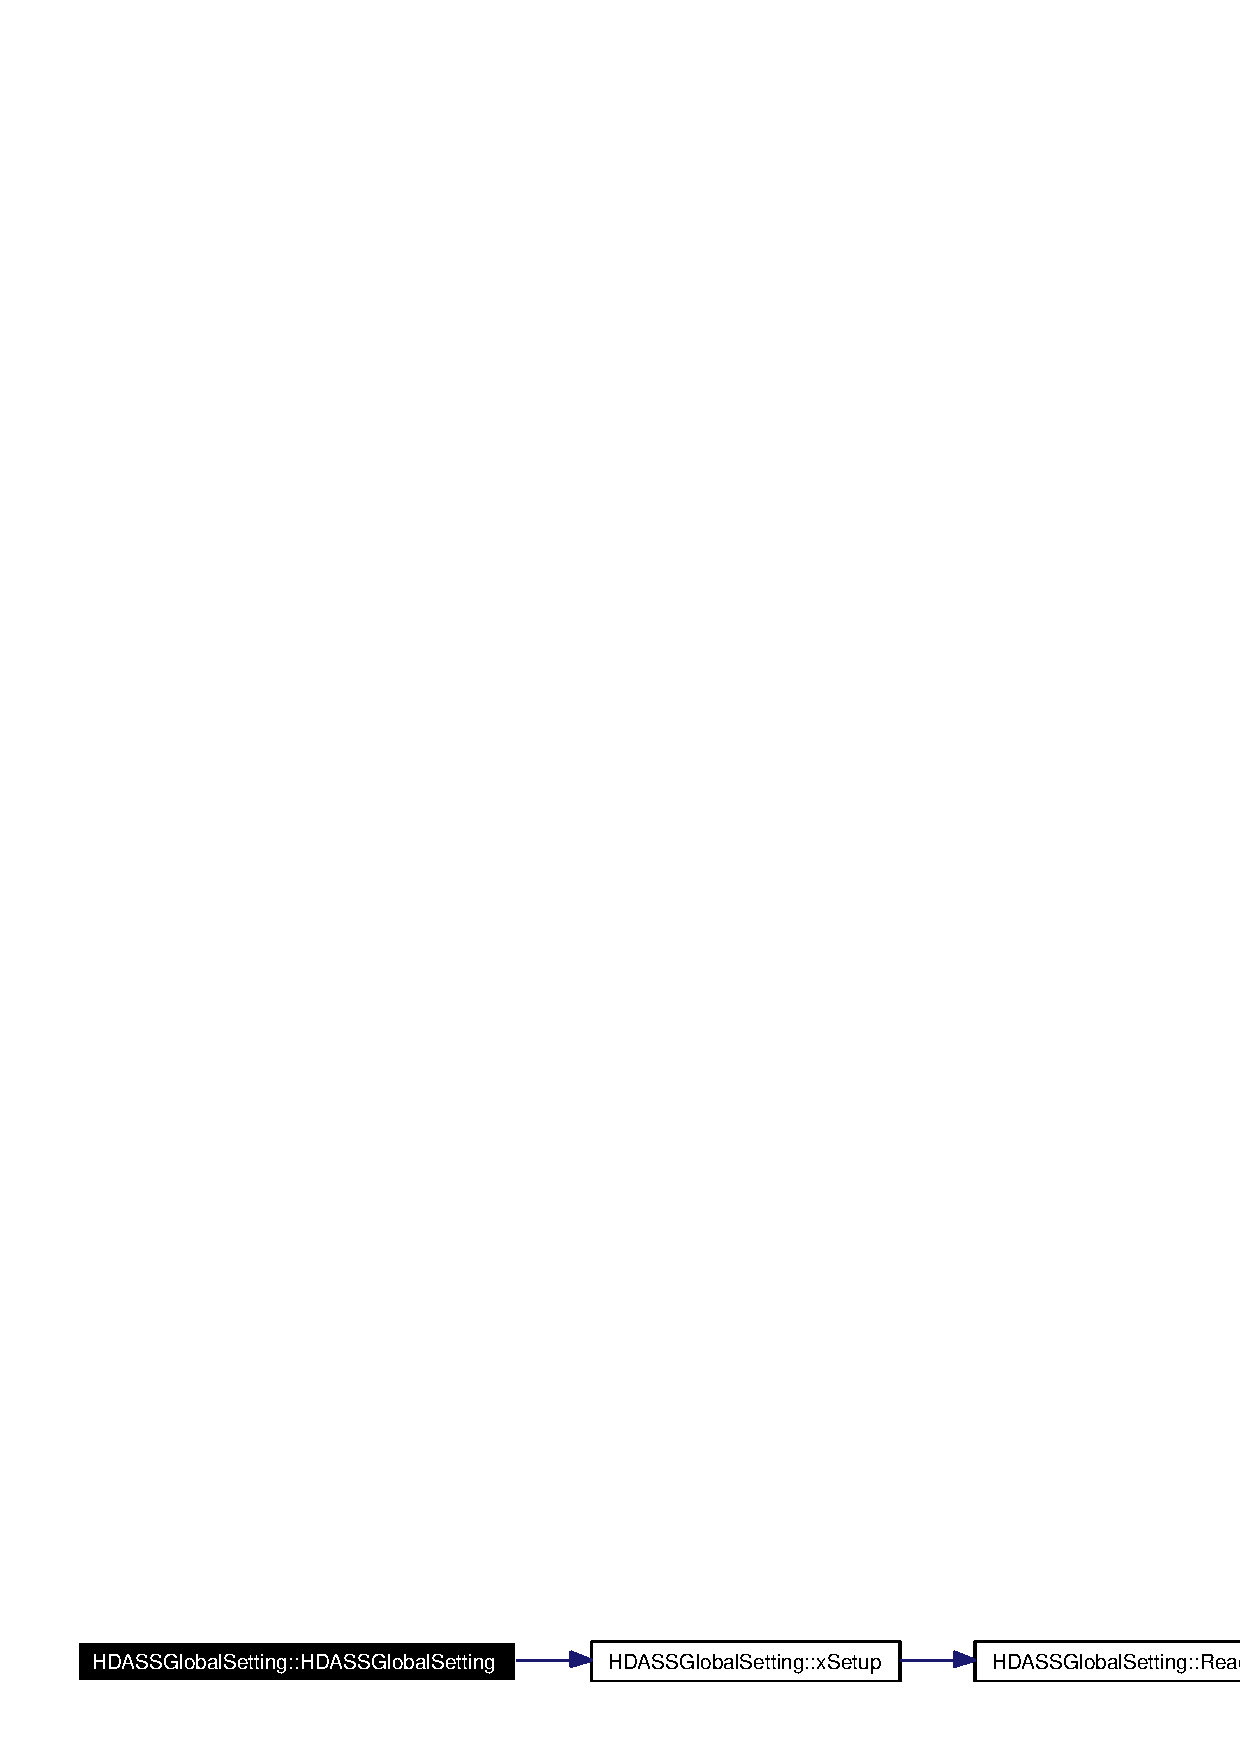
\includegraphics[width=329pt]{classHDASSGlobalSetting_HDASSGlobalSettinga0_cgraph}
\end{center}
\end{figure}
\index{HDASSGlobalSetting@{HDASSGlobal\-Setting}!~HDASSGlobalSetting@{$\sim$HDASSGlobalSetting}}
\index{~HDASSGlobalSetting@{$\sim$HDASSGlobalSetting}!HDASSGlobalSetting@{HDASSGlobal\-Setting}}
\subsubsection{\setlength{\rightskip}{0pt plus 5cm}HDASSGlobal\-Setting::$\sim${\bf HDASSGlobal\-Setting} ()}\label{classHDASSGlobalSetting_HDASSGlobalSettinga1}




Definition at line 29 of file hdassglobalsetting.cpp.



\footnotesize\begin{verbatim}30 {
31 }
\end{verbatim}\normalsize 


\subsection{Member Function Documentation}
\index{HDASSGlobalSetting@{HDASSGlobal\-Setting}!ReadingInitState@{ReadingInitState}}
\index{ReadingInitState@{ReadingInitState}!HDASSGlobalSetting@{HDASSGlobal\-Setting}}
\subsubsection{\setlength{\rightskip}{0pt plus 5cm}void HDASSGlobal\-Setting::Reading\-Init\-State ()}\label{classHDASSGlobalSetting_HDASSGlobalSettinga3}




Definition at line 38 of file hdassglobalsetting.cpp.

References em\_\-album, em\_\-display\_\-internet, em\_\-internet, int\-HDASS\_\-ALBUMCLOCK\_\-STATE, int\-HDASS\_\-FUNCTION\_\-STATE, int\-HDSS\_\-DISPLAY\_\-STATE, and List\-File\-Name.

Referenced by x\-Setup().



\footnotesize\begin{verbatim}39 {
40   //init  all needed here
41   intHDASS_FUNCTION_STATE=em_internet;
42   intHDASS_ALBUMCLOCK_STATE=em_album;
43   intHDSS_DISPLAY_STATE=em_display_internet;
44   //read from file
45   ListFileName=QString("PlayList.pls");
46 }
\end{verbatim}\normalsize 
\index{HDASSGlobalSetting@{HDASSGlobal\-Setting}!xSetup@{xSetup}}
\index{xSetup@{xSetup}!HDASSGlobalSetting@{HDASSGlobal\-Setting}}
\subsubsection{\setlength{\rightskip}{0pt plus 5cm}void HDASSGlobal\-Setting::x\-Setup ()}\label{classHDASSGlobalSetting_HDASSGlobalSettinga2}




Definition at line 33 of file hdassglobalsetting.cpp.

References Reading\-Init\-State().

Referenced by HDASSGlobal\-Setting().



\footnotesize\begin{verbatim}34 {
35   ReadingInitState();
36 }
\end{verbatim}\normalsize 


Here is the call graph for this function:\begin{figure}[H]
\begin{center}
\leavevmode
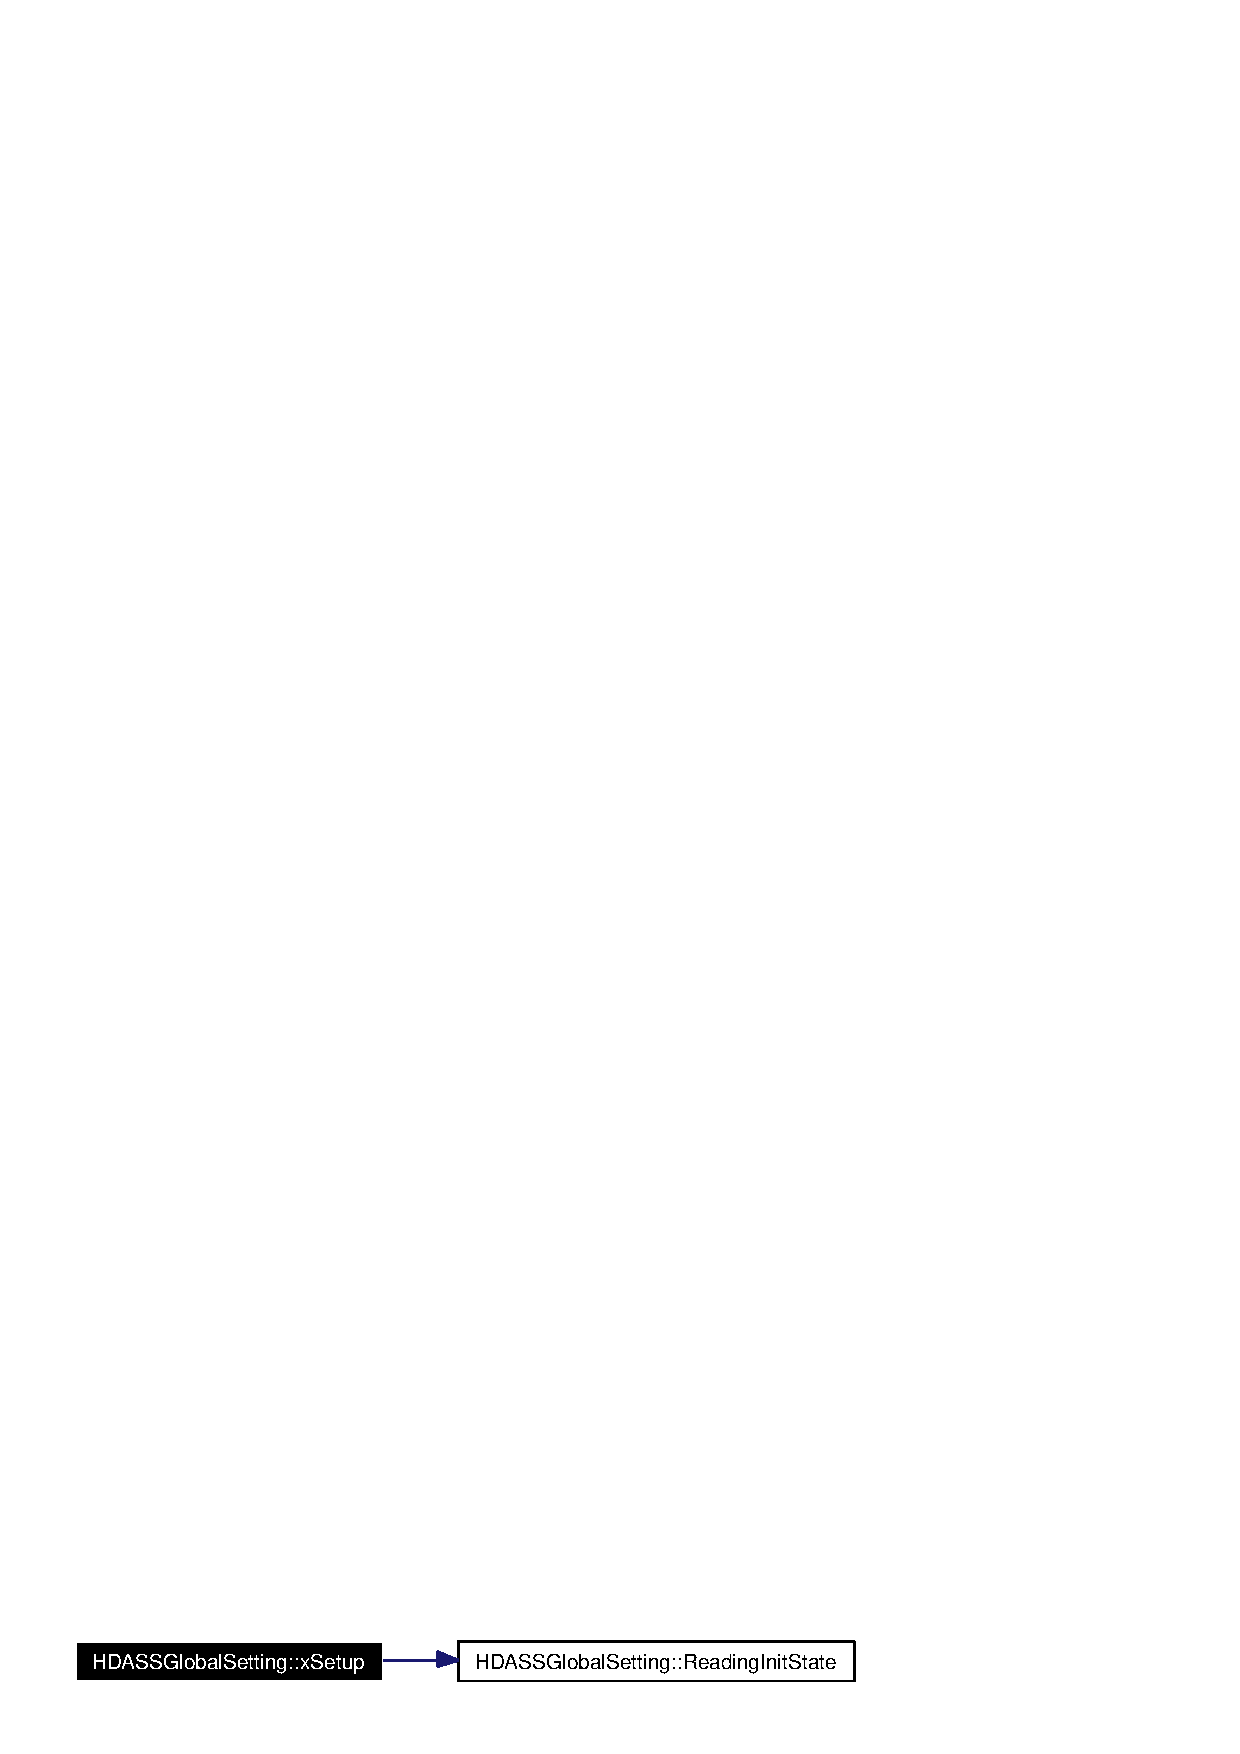
\includegraphics[width=205pt]{classHDASSGlobalSetting_HDASSGlobalSettinga2_cgraph}
\end{center}
\end{figure}


\subsection{Member Data Documentation}
\index{HDASSGlobalSetting@{HDASSGlobal\-Setting}!intHDASS_ALBUMCLOCK_STATE@{intHDASS\_\-ALBUMCLOCK\_\-STATE}}
\index{intHDASS_ALBUMCLOCK_STATE@{intHDASS\_\-ALBUMCLOCK\_\-STATE}!HDASSGlobalSetting@{HDASSGlobal\-Setting}}
\subsubsection{\setlength{\rightskip}{0pt plus 5cm}int {\bf HDASSGlobal\-Setting::int\-HDASS\_\-ALBUMCLOCK\_\-STATE}}\label{classHDASSGlobalSetting_HDASSGlobalSettingo1}




Definition at line 41 of file hdassglobalsetting.h.

Referenced by Reading\-Init\-State(), Function\-Bar::slot\-Change\-Function\-Sub\-Bar(), and Sub\-Bar\-Album\-Clock::slot\-Change\-Mode().\index{HDASSGlobalSetting@{HDASSGlobal\-Setting}!intHDASS_FUNCTION_STATE@{intHDASS\_\-FUNCTION\_\-STATE}}
\index{intHDASS_FUNCTION_STATE@{intHDASS\_\-FUNCTION\_\-STATE}!HDASSGlobalSetting@{HDASSGlobal\-Setting}}
\subsubsection{\setlength{\rightskip}{0pt plus 5cm}int {\bf HDASSGlobal\-Setting::int\-HDASS\_\-FUNCTION\_\-STATE}}\label{classHDASSGlobalSetting_HDASSGlobalSettingo0}




Definition at line 40 of file hdassglobalsetting.h.

Referenced by Reading\-Init\-State(), Function\_\-Control\_\-Area::slot\-Image\-Detial(), Function\_\-Control\_\-Area::slot\-Process\-Change\-Func(), Function\_\-Control\_\-Area::slot\-Show\-Image\-Detial(), Function\-Bar::x\-Setup(), and Function\_\-Control\_\-Area::x\-Setup().\index{HDASSGlobalSetting@{HDASSGlobal\-Setting}!intHDSS_DISPLAY_STATE@{intHDSS\_\-DISPLAY\_\-STATE}}
\index{intHDSS_DISPLAY_STATE@{intHDSS\_\-DISPLAY\_\-STATE}!HDASSGlobalSetting@{HDASSGlobal\-Setting}}
\subsubsection{\setlength{\rightskip}{0pt plus 5cm}int {\bf HDASSGlobal\-Setting::int\-HDSS\_\-DISPLAY\_\-STATE}}\label{classHDASSGlobalSetting_HDASSGlobalSettingo2}




Definition at line 42 of file hdassglobalsetting.h.

Referenced by Sub\-Bar\-Album\-Clock::Change\-Button\-Graphic(), Reading\-Init\-State(), Function\-Bar::slot\-Change\-Function\-Sub\-Bar(), Sub\-Bar\-Album\-Clock::slot\-Change\-Mode(), and Display\-Area::x\-Setup().\index{HDASSGlobalSetting@{HDASSGlobal\-Setting}!ListFileName@{ListFileName}}
\index{ListFileName@{ListFileName}!HDASSGlobalSetting@{HDASSGlobal\-Setting}}
\subsubsection{\setlength{\rightskip}{0pt plus 5cm}QString {\bf HDASSGlobal\-Setting::List\-File\-Name}}\label{classHDASSGlobalSetting_HDASSGlobalSettingo3}




Definition at line 43 of file hdassglobalsetting.h.

Referenced by Reading\-Init\-State(), hdassplaylist::Save\-List(), and hdassplaylist::x\-Setup().

The documentation for this class was generated from the following files:\begin{CompactItemize}
\item 
{\bf hdassglobalsetting.h}\item 
{\bf hdassglobalsetting.cpp}\end{CompactItemize}
